\documentclass[10pt,aspectratio=169,serif]{beamer}

\usepackage[fontset=none, scheme=plain]{ctex}
\IfFontExistsTF{Songti SC}{%
	\setCJKmainfont{Songti SC}[AutoFakeSlant=0.2]%
	\setCJKsansfont{Songti SC}[AutoFakeSlant=0.2]%
}{%
	\setCJKmainfont{FandolSong-Regular}[Extension=.otf,BoldFont=FandolSong-Bold,AutoFakeSlant=0.2]%
	\setCJKsansfont{FandolSong-Regular}[Extension=.otf,BoldFont=FandolSong-Bold]%
}
\usepackage{amsmath,amssymb,graphicx,tikz,booktabs,multicol,calligra}
\usepackage{pgfplots}
\pgfplotsset{compat=1.18}
\usepackage{tcolorbox}
\tcbuselibrary{skins}
\usepackage{XyygU}
\usepackage{caption}
\captionsetup[figure]{name=图,labelsep=period}

\usetikzlibrary{arrows.meta,positioning,calc}

\setlength{\abovedisplayskip}{0pt plus 2pt minus 2pt}
\setlength{\belowdisplayskip}{0pt plus 2pt minus 2pt}

\title[对数函数练习]{4.4 对数函数（练习）}
\subtitle{概念 \& 图象性质 \& 增长差异}
\author{}
\institute{}
\date{2026-10-16}

\begin{document}

\begin{frame}
  \titlepage
\end{frame}

% ========== 4.4.1 练习 第1题 ==========
\begin{frame}[t]{概念练习1：求函数定义域}
\textbf{1.} 求下列函数的定义域：

\vspace{0.5em}
\begin{columns}[t]
\begin{column}{0.5\textwidth}
\begin{enumerate}
  \item $y = \ln(1-x)$；
  \item $y = \dfrac{1}{\lg x}$；
\end{enumerate}
\end{column}
\begin{column}{0.5\textwidth}
\begin{enumerate}\setcounter{enumi}{2}
  \item $y = \log_7\dfrac{1}{1-3x}$；
  \item $y = \log_a |x|$（$a>0$，$a\neq 1$）。
\end{enumerate}
\end{column}
\end{columns}
\end{frame}

\begin{frame}[t]{概念练习1 解答}
\begin{tcolorbox}[colback=orange!10,colframe=orange,title=\textbf{解}]
(1) $1-x > 0 \Rightarrow x < 1$，定义域：$\alert{(-\infty,\,1)}$。

(2) $x>0$ 且 $\lg x \neq 0$，即 $x>0$ 且 $x\neq 1$，定义域：$\alert{(0,1)\cup(1,+\infty)}$。

(3) $1-3x > 0 \Rightarrow x < \dfrac{1}{3}$，定义域：$\alert{\left(-\infty,\,\dfrac{1}{3}\right)}$。

(4) $|x| > 0 \Rightarrow x \neq 0$，定义域：$\alert{(-\infty,0)\cup(0,+\infty)}$。
\end{tcolorbox}
\end{frame}

% ========== 概念练习 第2题 ==========
\begin{frame}[t]{概念练习2：画出函数图象}
\textbf{2.} 画出下列函数的图象：

\vspace{0.8em}
(1) $y = \lg 10^x$；

\vspace{0.8em}
(2) $y = 10^{\lg x}$。
\end{frame}

\begin{frame}[t]{概念练习2 解答}
\begin{tcolorbox}[colback=orange!10,colframe=orange,title=\textbf{解}]
(1) 对任意实数 $x$，$\lg 10^x = x$，所以 $y = \lg 10^x = x$，定义域为 $\mathbf{R}$，图象是直线 $y=x$。

(2) 由对数定义，$10^{\lg x} = x$，但需 $x>0$（$\lg x$ 有意义），所以 $y = 10^{\lg x} = x$（$x>0$），图象是直线 $y=x$ 在 $y$ 轴右侧的部分（不含原点）。
\end{tcolorbox}
\end{frame}

\begin{frame}[t]{概念练习2 图象}
\begin{center}
\begin{tikzpicture}[scale=0.9]
\begin{axis}[
    width=10cm, height=7cm,
    axis lines=middle,
    xlabel=$x$, ylabel=$y$,
    xmin=-3, xmax=4, ymin=-3, ymax=4,
    xtick={-2,2}, ytick={-2,2},
    grid=major, grid style={gray!20},
]
% y=x 完整直线
\addplot[thick,blue,domain=-3:4,samples=2] {x};
\node[blue] at (axis cs:2.5,2.8) {$y=x$（全体实数）};
% 右侧射线（2）
\addplot[very thick,red,domain=0:4,samples=2] {x};
\node[red] at (axis cs:3,3.4) {$y=x$（$x>0$）};
\end{axis}
\end{tikzpicture}
\end{center}
\end{frame}

% ========== 概念练习 第3题 ==========
\begin{frame}[t]{概念练习3：函数关系判断}
\textbf{3.} 已知集合 $A = \{1, 2, 3, 4, \cdots\}$，集合 $B = \{2, 4, 6, 8, 10, \cdots\}$，下列表达式能建立从集合 $A$ 到集合 $B$ 的函数关系的是 \underline{\hspace{2em}}。

\vspace{1em}
\hspace{2em}① $y = 2^x$；\hspace{2em}② $y = x^2$；\hspace{2em}③ $y = \log_2 x$；\hspace{2em}④ $y = 2x$。
\end{frame}

\begin{frame}[t]{概念练习3 解答}
\begin{tcolorbox}[colback=orange!10,colframe=orange,title=\textbf{解}]
判断：对任意 $x\in A$，函数值 $y$ 是否都属于 $B$。

\vspace{0.3em}
① $y=2^x$：$1\to 2$，$2\to 4$，$3\to 8$，$4\to 16$，$\cdots$ 都是偶数，在 $B$ 中。\alert{是}。

② $y=x^2$：$1\to 1$，而 $1\notin B$。\alert{不是}。

③ $y=\log_2 x$：$1\to 0$，而 $0\notin B$。\alert{不是}。

④ $y=2x$：$1\to 2$，$2\to 4$，$3\to 6$，$\cdots$ 都是正偶数，在 $B$ 中。\alert{是}。

\vspace{0.3em}
\alert{答案：①④}。
\end{tcolorbox}
\end{frame}

% ========== 4.4.2 练习 第1题 ==========
\begin{frame}[t]{图象练习1：画 $y=\log_3 x$ 和 $y=\log_{1/3} x$}
\textbf{1.} 在同一直角坐标系中画出函数 $y = \log_3 x$ 和 $y = \log_{\frac{1}{3}} x$ 的图象，并说明它们的关系。
\end{frame}

\begin{frame}[t]{图象练习1 解答与图象}
\begin{tcolorbox}[colback=orange!10,colframe=orange,title=\textbf{解}]
因为 $\log_{\frac{1}{3}} x = -\log_3 x$，所以点 $(x, y)$ 与 $(x, -y)$ 关于 $x$ 轴对称。

\vspace{0.3em}
因此，$y = \log_{\frac{1}{3}} x$ 的图象与 $y = \log_3 x$ 的图象关于 \alert{$x$ 轴对称}。
\end{tcolorbox}

\begin{center}
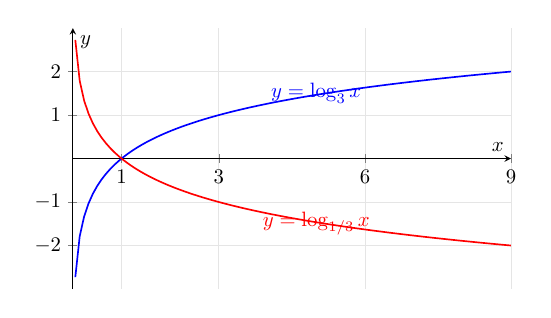
\begin{tikzpicture}[scale=0.75]
\begin{axis}[
    width=9cm, height=6cm,
    axis lines=middle,
    xlabel=$x$, ylabel=$y$,
    xmin=0, xmax=9, ymin=-3, ymax=3,
    xtick={1,3,6,9}, ytick={-2,-1,1,2},
    grid=major, grid style={gray!20},
]
\addplot[thick,blue,domain=0.05:9,samples=100] {ln(x)/ln(3)};
\node[blue] at (axis cs:5,1.5) {$y=\log_3 x$};
\addplot[thick,red,domain=0.05:9,samples=100] {-ln(x)/ln(3)};
\node[red] at (axis cs:5,-1.5) {$y=\log_{1/3} x$};
\end{axis}
\end{tikzpicture}
\end{center}
\end{frame}

% ========== 图象练习 第2题 ==========
\begin{frame}[t]{图象练习2：比较大小}
\textbf{2.} 比较下列各题中两个值的大小：

\vspace{0.5em}
\begin{enumerate}
  \item $\lg 0.6$，$\lg 0.8$；
  \item $\log_{0.5} 6$，$\log_{0.5} 4$；
  \item $\log_m 5$，$\log_m 7$。
\end{enumerate}
\end{frame}

\begin{frame}[t]{图象练习2 解答}
\begin{tcolorbox}[colback=orange!10,colframe=orange,title=\textbf{解}]
(1) $y=\lg x$ 在 $(0,+\infty)$ 上是增函数，$0.6<0.8$，所以 $\alert{\lg 0.6 < \lg 0.8}$。

(2) 底数 $0.5<1$，$y=\log_{0.5} x$ 是减函数，$6>4$，所以 $\alert{\log_{0.5} 6 < \log_{0.5} 4}$。

(3) 需对底数 $m$ 分类讨论：

\hspace{2em}当 $m>1$ 时，$y=\log_m x$ 是增函数，$5<7$，所以 $\log_m 5 < \log_m 7$；

\hspace{2em}当 $0<m<1$ 时，$y=\log_m x$ 是减函数，$5<7$，所以 $\log_m 5 > \log_m 7$。
\end{tcolorbox}
\end{frame}

% ========== 图象练习 第3题 ==========
\begin{frame}[t]{图象练习3：GDP增长}
\textbf{3.} 某地去年的GDP为 $3000$ 亿元人民币，预计未来 $5$ 年的平均增长率为 $6.8\%$。

\vspace{0.5em}
(1) 设经过 $x$ 年达到的年GDP为 $y$ 亿元，试写出未来 $5$ 年内，$y$ 关于 $x$ 的函数解析式；

(2) 经过几年该地GDP能达到 $3900$ 亿元人民币？
\end{frame}

\begin{frame}[t]{图象练习3 解答}
\begin{tcolorbox}[colback=orange!10,colframe=orange,title=\textbf{解}]
(1) $y = 3000(1+6.8\%)^x = 3000\times 1.068^x$，$x\in [0, 5]$。

(2) 令 $3000\times 1.068^x = 3900$，则 $1.068^x = 1.3$。
\[
x = \log_{1.068} 1.3 = \frac{\lg 1.3}{\lg 1.068} \approx \frac{0.1139}{0.0286} \approx 4.0.
\]
所以大约经过 $\alert{4}$ 年该地GDP能达到 $3900$ 亿元。
\end{tcolorbox}
\end{frame}

% ========== 4.4.3 练习 第1题 ==========
\begin{frame}[t]{增长差异练习1：判断指数增长}
\textbf{1.} 三个变量 $y_1, y_2, y_3$ 随变量 $x$ 变化的数据如下表。其中关于 $x$ 呈指数增长的变量是 \underline{\hspace{2em}}。

\vspace{0.5em}
\begin{center}
\begin{tabular}{c|ccccccc}
$x$ & 0 & 5 & 10 & 15 & 20 & 25 & 30\\
\hline
$y_1$ & 5 & 130 & 505 & 1130 & 2005 & 3130 & 4505\\
$y_2$ & 5 & 90 & 1620 & 29160 & 524880 & 9447840 & 170061120\\
$y_3$ & 5 & 30 & 55 & 80 & 105 & 130 & 155
\end{tabular}
\end{center}
\end{frame}

\begin{frame}[t]{增长差异练习1 解答}
\begin{tcolorbox}[colback=orange!10,colframe=orange,title=\textbf{解}]
\textbf{$y_3$}：相邻两项差恒为 $25$，呈\alert{线性增长}（一次函数）。

\textbf{$y_1$}：增量依次为 $125, 375, 625, 875, 1125, 1375$，二次差恒为 $250$，呈\alert{二次增长}。

\textbf{$y_2$}：相邻两项比值约为 $18, 18, 18, 18, 18, 18$（恒定倍数），呈\alert{指数增长}。

\vspace{0.5em}
\alert{答案：$y_2$}。
\end{tcolorbox}
\end{frame}

% ========== 增长差异练习 第2题 ==========
\begin{frame}[t]{增长差异练习2：估算 $3^x > 5x$ 的范围}
\textbf{2.} 借助计算工具估算出使 $3^x > 5x$ 的 $x$ 的取值范围（精确到 $0.01$）。
\end{frame}

\begin{frame}[t]{增长差异练习2 解答}
\begin{tcolorbox}[colback=orange!10,colframe=orange,title=\textbf{解}]
求方程 $3^x = 5x$ 的根：

\vspace{0.3em}
第一个根：在 $x=0.25$ 附近，$3^{0.25}\approx 1.316 > 1.25 = 5\times 0.25$；
在 $x=0.28$ 附近，$3^{0.28}\approx 1.36 < 1.4 = 5\times 0.28$。
故第一个根约为 $\alert{x \approx 0.27}$。

\vspace{0.3em}
第二个根：在 $x=2.15$ 附近，$3^{2.15}\approx 10.61 < 10.75 = 5\times 2.15$；
在 $x=2.2$ 附近，$3^{2.2}\approx 11.21 > 11 = 5\times 2.2$。
故第二个根约为 $\alert{x \approx 2.18}$。

\vspace{0.3em}
因此 $3^x > 5x$ 的解集为 $\alert{(-\infty,\,0.27)\cup(2.18,\,+\infty)}$。
\end{tcolorbox}
\end{frame}

\begin{frame}[t]{增长差异练习2 图象}
\begin{center}
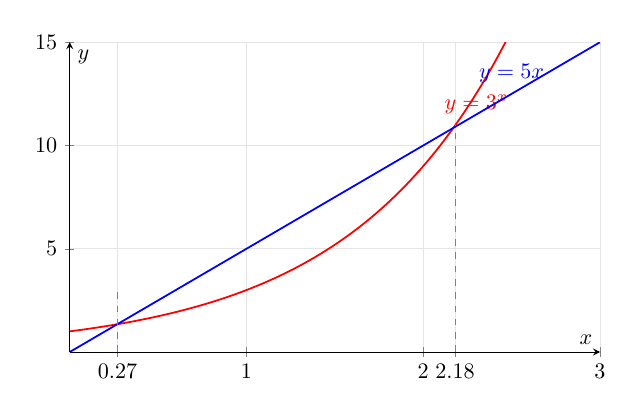
\begin{tikzpicture}[scale=0.8]
\begin{axis}[
    width=10cm, height=6.5cm,
    axis lines=middle,
    xlabel=$x$, ylabel=$y$,
    xmin=0, xmax=3, ymin=0, ymax=15,
    xtick={0.27,1,2,2.18,3}, ytick={5,10,15},
    grid=major, grid style={gray!20},
]
\addplot[thick,red,domain=0:3,samples=100] {3^x};
\node[red] at (axis cs:2.3,12) {$y=3^x$};
\addplot[thick,blue,domain=0:3,samples=2] {5*x};
\node[blue] at (axis cs:2.5,13.5) {$y=5x$};
\draw[dashed,gray] (axis cs:0.27,0) -- (axis cs:0.27,3);
\draw[dashed,gray] (axis cs:2.18,0) -- (axis cs:2.18,11);
\end{axis}
\end{tikzpicture}
\end{center}
\end{frame}

% ========== 增长差异练习 第3题 ==========
\begin{frame}[t]{增长差异练习3：求一次函数解析式}
\textbf{3.} 如图，对数函数 $y = \lg x$ 的图象与一次函数 $y = f(x)$ 的图象有 $A$，$B$ 两个公共点。已知 $A(1, 0)$，$B$ 点的横坐标为 $2$。求一次函数 $y = f(x)$ 的解析式。

\vspace{1em}
\begin{center}
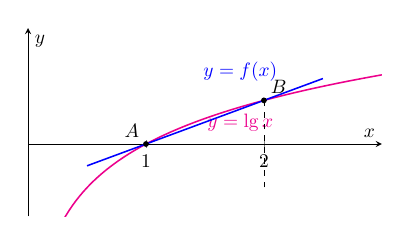
\begin{tikzpicture}[scale=0.7]
\begin{axis}[
    width=8cm, height=5cm,
    axis lines=middle,
    xlabel=$x$, ylabel=$y$,
    xmin=0, xmax=3, ymin=-0.5, ymax=0.8,
    xtick={1,2}, ytick={0},
]
\addplot[thick,magenta,domain=0.05:3,samples=100] {ln(x)/ln(10)};
\node[magenta] at (axis cs:1.8,0.15) {$y=\lg x$};
\addplot[thick,blue,domain=0.5:2.5,samples=2] {(ln(2)/ln(10))*(x-1)};
\node[blue] at (axis cs:1.8,0.5) {$y=f(x)$};
\fill (axis cs:1,0) circle (1.5pt);
\node[above left] at (axis cs:1,0) {$A$};
\fill (axis cs:2,{ln(2)/ln(10)}) circle (1.5pt);
\node[above right] at (axis cs:2,{ln(2)/ln(10)}) {$B$};
\draw[dashed] (axis cs:2,-0.3) -- (axis cs:2,{ln(2)/ln(10)});
\end{axis}
\end{tikzpicture}
\end{center}
\end{frame}

\begin{frame}[t]{增长差异练习3 解答}
\begin{tcolorbox}[colback=orange!10,colframe=orange,title=\textbf{解}]
$A(1, 0)$ 在 $y=\lg x$ 上（$\lg 1 = 0$）。

$B$ 点横坐标为 $2$，且在 $y=\lg x$ 上，所以 $B(2, \lg 2)$。

\vspace{0.3em}
一次函数 $f(x)$ 过 $(1, 0)$ 和 $(2, \lg 2)$，斜率 $k = \dfrac{\lg 2 - 0}{2 - 1} = \lg 2$。

\vspace{0.3em}
所以：
\[
\alert{f(x) = (\lg 2)(x - 1)}.
\]
\end{tcolorbox}
\end{frame}

% ========== 增长差异练习 第4题 ==========
\begin{frame}[t]{增长差异练习4：选择合适的函数}
\textbf{4.} 函数 $y = f(x)$ 的图象过 $(1, 0)$，在 $(0,+\infty)$ 上单调递增，且以 $y=1$ 为水平渐近线。则 $y = f(x)$ 可能是（\quad）。

\vspace{0.5em}
\begin{columns}[t]
\begin{column}{0.5\textwidth}
\begin{enumerate}[(A)]
  \item $y = 1 - x^{-1}$，$x\in(0,+\infty)$；
  \item $y = \dfrac{3}{2} - \left(\dfrac{1}{2}\right)^x$，$x\in(0,+\infty)$；
\end{enumerate}
\end{column}
\begin{column}{0.5\textwidth}
\begin{enumerate}[(A)]\setcounter{enumi}{2}
  \item $y = \ln x$；
  \item $y = x - 1$，$x\in(0,+\infty)$。
\end{enumerate}
\end{column}
\end{columns}
\end{frame}

\begin{frame}[t]{增长差异练习4 解答}
\begin{tcolorbox}[colback=orange!10,colframe=orange,title=\textbf{解}]
逐一验证：

\vspace{0.3em}
(A) $y=1-\dfrac{1}{x}$：$x=1$ 时 $y=0$；$x\to 0^+$ 时 $y\to -\infty$；$x\to+\infty$ 时 $y\to 1$（以 $y=1$ 为渐近线）。\alert{符合}。

(B) $y=\dfrac{3}{2}-\left(\dfrac{1}{2}\right)^x$：$x=0$ 时 $y=\dfrac{1}{2}$，渐近线 $y=\dfrac{3}{2}$。不符合。

(C) $y=\ln x$：$x\to+\infty$ 时 $y\to+\infty$，无水平渐近线。不符合。

(D) $y=x-1$：是直线，无水平渐近线。不符合。

\vspace{0.3em}
\alert{答案：(A)}。
\end{tcolorbox}
\end{frame}

\begin{frame}[c]
  \begin{center}
    {\Huge\calligra Thanks!}
  \end{center}
\end{frame}

\end{document}
